
\documentclass[a4paper, oneside, 11pt]{report}
\usepackage{epsfig,pifont,float,multirow,amsmath,amssymb}
\newcommand{\mc}{\multicolumn{1}{c|}}
\newcommand{\mb}{\mathbf}
\newcommand{\mi}{\mathit}
\newcommand{\oa}{\overrightarrow}
\newcommand{\bs}{\boldsymbol}
\newcommand{\ra}{\rightarrow}
\newcommand{\la}{\leftarrow}
\usepackage{algorithm}
\usepackage{algorithmic}
\topmargin = 0pt
\voffset = -80pt
\oddsidemargin = 15pt
\textwidth = 425pt
\textheight = 750pt

\begin{document}

\begin{titlepage}
\begin{center}
\rule{12cm}{1mm} \\
\vspace{1cm}
{\large  CMP-6048A Advanced Programming}
\vspace{7.5cm}
\\{\Large Project Report - 10 January 2024}
\vspace{1.5cm}
\\{\LARGE MATBAP: Maths Interpreter software}
\vspace{1.0cm}
\\{\Large Group members: \\ Igor Stepanenko, Lyra, Liam Farese\ }
\vspace{10.0cm}
\\{\large School of Computing Sciences, University of East Anglia}
\\ \rule{12cm}{0.5mm}
\\ \hspace{8.5cm} {\large Version 2.0}
\end{center}
\end{titlepage}


\setcounter{page}{1}
%\pagenumbering{roman}
%\newpage


\begin{abstract}
Please replace this section with your own abstract. An abstract is a brief summary (maximum 250 words) of your entire project. It should cover your objectives, your methodologies used, a brief developmental history, your final results, in particular covering the optional tasks, and a discussion and conclusion. You do not cover the literature or background in an abstract nor should you use abbreviations or acronyms. The remainder of this report template has clear chapter titles and we suggest to stick to these although you can organise your material inside each chapter to your own preferences. A guideline in size is approximately 3,500 words (not including abstract, captions and references) but no real limit on figures, tables, diagrams, pseudo-code etc.
\end{abstract}

\chapter{Introduction}
\label{chap:intro}

\section{Project statement}
This project will be a Maths Interpreter software with extensions aiming
towards a Turing complete language. It will be used to evaluate expressions, define
variables and functions, and plot functions of two variables. The software
will allow the user to enter expressions and equations using a custom language which is processed by a lexer, parser and evaluator. Plots of mathematical equations will be interactive. Additional functionality might include root finding, differentiation and integration. The software will be developed keeping in mind software engineering principles such as low coupling and high cohesion achieved through Model-View-ViewModel and Inversion of Control patterns. 

\section{Aims and objectives}
The main aim is to develop Matbap, a maths interpreter software for solving and plotting mathematical expressions. Main objectives include:
\begin{itemize}
    \item Create Lexer, Parser and Evaluator in F\# to process mathematical expressions and equations to plot.
    \item Develop a Graphical User Interface (GUI) in C\# for user interaction.
    \item Integrate F\# and C\# components keeping in mind low coupling.
\end{itemize}

\noindent % Start a new paragraph without indentation
They are broken further into subtasks in this MoSCoW table \ref{appendix:moscow} 


\chapter{Background}
The development of maths software capable of plotting graphs has become significantly easier in recent years, because of integration of technology in education and research. Therefore, it is important we acknowledge key software and literature in this field.

Desmos\cite{Desmos:2023} software offers a graphical calculator that changed the way students learn mathematics by providing an intuitive UI and robust plotting functionality to allow for visualisations of complex functions and equations.

MATLAB\cite{Matlab:2023} is the mainstream tool in the field of mathematical computing, visualising and programming. It offers extensive tooling that includes signal and image processing, which is why it is widely used in academia and industry.

The Windows Presentation Foundation (WPF)\cite{WPF:2023} documentation provided by Microsoft Learn offered tutorials and guidance on creating desktop user interfaces. WPF’s powerful data-bindings were critical in displaying mathematical data back to the user.

The Dependency Injection (DI) \cite{DI:2023} documentation from Microsoft Learn described the design pattern that produces more testable and modular software. In the context of our application, this pattern allowed for dynamic integration of different services like equation evaluator and plotting evaluator, and as a result made our software more maintainable and scalable.

The Model-View-ViewModel (MVVM)\cite{MVVM:2022} documentation from Microsoft Learn describes the architecture, which is primarily used with WPF applications due to its powerful data-binding features. MVVM creates a clear separation of concerns where business logic is decoupled from the UI. This architecture was important in developing our software because it allowed for maintainable and scalable code, which could handle mathematical calculations and user interactions.


\chapter{Development History}\label{Chap:DevHist}

\section{Sprint 0: Setup development infrastructure}
At the very start of this project, we needed to setup and integrate essentials tools that have been critical in streamlining workflow and improving teamwork.

\subsection{Jira Board}
To track our work, we chose Jira\cite{Atlassian:JIRA} - tool for task management and sprint planning, which provided us with visual representation of our project's progress. We setup a Jira Board(link \ref{ap-jira-link}) that helped us create a backlog tickets, that can be assigned to a team member and tracked in To Do, In Progress and Done columns.

\subsection{Visual Studio Project}
Next we configured a Visual Studio solution that could reference a F\# application in a C\# application as a DLL\cite{DLL}.

\subsection{GitHub repository}
We setup a version a control system for our codebase - GitHub repository(link - \ref{github-repo}). This enabled us to collaborate, peer review each others work and keep a history of contributions to the project. A significant objective was to setup a Continuous Integration (CI)\cite{Atlassian:CI} using GitHub Actions\cite{GitHubDocs:Actions} to ensure that our codebase remains bug free through automated testing before any changes are merged to the main branch.

\subsection{Conclusion}
This sprint has laid foundation to our development journey. Setting up tools like Jira, GitHub and Visual Studio not only streamlined our workflow but also enabled us to be an effective and efficient team.

% https://liamfarese.atlassian.net/browse/AP-8
\section{Sprint 1: Basic arithmetic calculations, Basic GUI.}
In our first sprint, we focused on building the foundation of our maths interpreter, like basic arithmetic calculations and basic GUI. Our objective was to develop a software that mathces the spec requirements and is a robust and scalable application, keeping in mind maintainability and testability.

\subsection{Lexer}
We developed a lexer that would tokenise expressions consisting of digits, binary operations, identifiers and functions like sin, cos and tan. One of the challenges we faced was unfamiliarity with F\# and functional programming, especially the recursive nature of this programming paradigm. 

\subsection{Parser}
We developed a parser that would parse and evaluate expressions that followed this basic grammar.
\begin{verbatim}
 <E>    ::= <T> <Eopt>
 <Eopt> ::= + <T> <Eopt> | - <T> <Eopt> | <empty>
 <T>    ::= <NR> <Topt>
 <Topt> ::= * <NR> <Topt> | / <NR> <Topt> | <empty>
 <NR>   ::= <int> | <float> | (E)
\end{verbatim}

\subsection{Basic GUI}
We used WPF\cite{WPF:2023} with C\# to develop a basic GUI, focusing on maintainability, testability, and scalability. App's architecture consists of several design patterns like Model-View-ViewModel\cite{MVVM:2022}, that improves GUI's responsiveness to user interactions and Dependency Injection\cite{DI:2023} for better modularity and easy maintenance. The GUI was a minimalistic interface allowing users to enter expressions and view the answers - see Figure \ref{basicgui}.

\subsection{Testing}
Thorough unit tests were written for both the C\# app and the F\# engine. Table \ref{sprint1-lexer-test} includes unit test for the Lexer. Table \ref{sprint1-parser-test} includes unit tests for the Parser. The table with GUI unit tests can be seen in \ref{sprint1-gui-test}. The use of the MVVM and Dependency Injection patterns allowed us to to use the Moq\cite{Moq} mocking library to mock Model behaviours in our ViewModel. This allowed us to test code in isolation without relying on behaviour of real dependencies and to have control over what is returned from the mocked methods. As a result our code coverage was above 80\%.

\subsection{Conclusion}
The first sprint laid a solid foundation for our maths interpreter. The lexer and parser were capable of evaluation basic arithmetic expressions and the GUI was providing simple interface for user interaction. Our testing strategy set a ensured that future features were build upon a reliable codebase. 

%https://liamfarese.atlassian.net/browse/AP-30
\section{Sprint 2: Modulo and Power, Correct treatment of integers and floats, Help Menu, Lexer error handling, Link C\# app with F\# engine}

In our second sprint, we focused on improving functionality and user experience of our maths interpreter. Key improvements were support for modulo and power operators, correct handling of integers and floats, better errors in the Lexer and linking our GUI with the interpreter.

\subsection{Lexer}
We updated our lexer with better errors. Now it returns error messages that include the problematic token and its position. This improvement helped us in our debugging processes and provided more clarity to users.

\subsection{Parser}
After a review from the teaching team, we identified a bug. We didn't correctly handle our floats and integers. Previously, integers were cast to floats in order to allow calculation with them. Our fix allowed integers and floats to be handled separately: integer operations would always return integers and the same would happen for floats. The updated BNF reflects this change:
\begin{verbatim}
<E>    ::= <T> <Eopt>
<Eopt> ::= + <T> <Eopt> | - <T> <Eopt> | <empty>
<T>    ::= <NR> <Topt>
<Topt> ::= * <NR> <Topt> | / <NR> <Topt> | <empty>
<NR>   ::= <num> | (E)
<num>  ::= <int> | <float>
\end{verbatim}

Furthermore, we added support for modulo (\%) and power (\textasciicircum) operators. This is reflected in this updated BNF:
\begin{verbatim}
<E>    ::= <T> <Eopt>
<Eopt> ::= + <T> <Eopt> | - <T> <Eopt> | <empty>
<T>    ::= <P> <Topt>
<Topt> ::= * <P> <Topt> | / <P> <Topt> | % <P> <Topt> | <empty>
<P>    ::= <NR> <Popt>
<Popt> ::= ^ <NR> <Popt> | <empty>
<NR>   ::= <num> | (E)
<num>  ::= <int> | <float>
\end{verbatim}


\subsection{Updated GUI}
The GUI was updated with a Help window, that showed all supported tokens. This addition improved user accessibility. The connection of our GUI to our interpreter allowed for real time calculations. The screenshot of updated GUI can be seen in TODO \ref{helpgui}.

\subsection{Testing}
We updated our unit tests to validate new features and fixed bugs. They can be seen under TODO\ref{}

\subsection{Conclusion}
Sprint 2 has made good progress in developing our maths interpreter. The introduction of new operators and the correction of behaviour around integer and floats improved our app's versatility and better matched requirements. The lexer's errors and updated GUI improved user experience.


% https://liamfarese.atlassian.net/browse/AP-42
\section{Sprint 3: Unary minus, Assign variables, Plotting lines and polynomials}
In the third sprint we focused on extending our app’s functionality to support unary minus, variable assignments, and basic plotting functionality. These improvements aimed to increase app’s versatility, aligning with our goal to build a Maths Interpreter.

\subsection{Lexer}
We have updated our Lexer to recognise an assignment operator. The addition was critical to allow variable assignment functionality, allowing users to create and manipulate variables in their expressions. The implementation was to add a ‘=‘ operator to our set of tokens.

\subsection{Parser}
(Liam/Lyra - how it was done and discuss any key challenges or optimisations implemented/needed)

\subsection{Updated GUI}
To allow for basic plotting, we introduced a new Plotting Mode in the GUI. User could input equations, define x range and step. As a result of this change, we introduced new plotting ViewModel and View. We decided to use OxyPlot\cite{Oxyplot} - a popular plotting library in C\#, because of its ease of use. The ViewModel was full of code interacting with F\# engine, setting up OxyPlot plot model and generating line series for the function. However, we later realised that this design was flawed due to its scalability limitations and maintainability struggle, which we will fix in the future sprints. You can see new GUI under Appendix \ref{app:gui}.

\subsection{Testing}
Unit tests were added to cover all aspects of new features. These tests ensured correct implementations of unary minus, variable assignment and ViewModel’s interactions with F\# engine and View. These tests are in the table that can be found under Appendix \ref{app:test}.


\subsection{Conclusion}
This sprint has made great progress towards meeting all compulsory objectives tasks we had outlined in our MoSCoW table. Introduction of variable assignment and unary minus laid the foundation for plotting and future advanced features.



% https://liamfarese.atlassian.net/browse/AP-50
\section{Sprint 4: AST Parser and AST Evaluator}
While researching advanced features, we quickly realised we are very limited to what we can do with our F\# engine because it does not create an Abstract Syntax Tree (AST) and as a result we would struggle to add advanced features. In this sprint, we decided to refactor our Parser and Evaluator to construct and evaluate an AST.

\subsection{Parser}
Our strategy was to incrementally build a new parser. We started with integrating simple grammar from our existing BNF. Next we have implemented operators like power, modulo and unary minus. The last addition was variable assignment. This resulted in a fully functional parser that builds an AST of the expression. One of the crucial things we have almost missed was that the requirement for power operations to be right-associative. We were able to catch that using our extensive unit tests framework.
(Liam, please expand on the variable assignment parsing challenges and solutions.)
\begin{verbatim}
    
The AST Node type looked like this:
        type NumType =
            | Int of int
            | Float of float

       type Node =
            | Number of NumType
            | BinaryOperation of string * Node * Node
            | ParenthesisExpression of Node
            | UnaryMinusOperation of string * Node
            | VariableAssignment of string * Node
            | Variable of string
\end{verbatim}
\subsection{AST Evaluator}
(TODO: Lyra - how the evaluator was adapted to work with the AST and discuss any key challenges or optimisations implemented/needed)

\subsection{Testing}
Our unit tests written for the Parser were extensive to ensure correct AST is generated. They included testing for
\begin{itemize}
    \item correct integer and float nodes are created, 
    \item accurate nodes for simple and combined arithmetic operations, and nested parenthesis,
    \item accurate handling of power, modulo, and unary minus operations, 
    \item variables and variable assignment. 
\end{itemize}
The tests can be seen under Appendix \ref{app:test}.

(Lyra to add unit tests table to appendix and description for AST Evaluator unit tests.)

\subsection{Conclusion}
In this sprint we have made a massive refactor to transition to an AST architecture for parsing and evaluating stages. This not only solved our limitation issue, but also opened the doors to implement several advanced features.

\section{Sprint 5: Visualise parse tree, Multiple plots, Plotted functions table}
During this sprint, we continued to focus on improving our app's functionality. With introduction of the Abstract Syntax Tree Parser we set out to complete several optional objectives, such as visualising the parse tree, enabling users to plot multiple graphs and displaying all plotted function in a user-friendly table.

\subsection{Visualising parse tree}
Introduction of the Abstract Syntax Tree parser resulted in implementation of a converter between F\# and C\# for visualisation. We have introduced an abstract class $ASTNode$ and a converter class $ASTManager$. For the visualisation, we opted for Microsoft Automatic Graph Layout\cite{MSAGL} - a popular library used to display graph data structures, which we have adapted to display our Abstract Syntax Tree. The visualisation provides clarity for developers and users about the underlying parsing process. The resulting GUI can be seen under Appendix \ref{app:gui}.

\subsection{Adding multiple plots, Clearing plot area, Displaying plotted functions}
Anticipating more complex plotting functionality like adding tangents, we decided to extend our plotting mode to support adding multiple plots. The key change was refactoring our PlotViewModel to store a single instance of the OxyPlot's plot model. We also added a button to clear the plotting area to improve interface's flexibility and user experience. 

The ability to add multiple plots to the plot area introduced potential user confusion. To solve this issue, we implemented a feature to display all plotted functions, allowing users to select a plot to perform an operation like adding a tangent. This features involved storing all plots in a map, that could be displayed in the GUI using WPF's powerful data template and data binding features. The resulted GUI can be seen under Appendix \ref{app:gui}.

\subsection{Testing}
In this sprint, we concentrated our testing on new functionalities like $ASTManager$ class correctly converting F\# nodes to C\# nodes. The tests can be found under Appendix \ref{app:test}.

\subsection{Conclusion}
In this sprint we have added an advanced feature like Visualising the parse tree and laid a solid foundation for future work by enabling plotting multiple functions.

\section{Sprint 6: Differentiation, Adding tangents, Plotted function table}
In this sprint, we tackled maths toolbox objective, specifically Differentiation. This addition aimed at expanding our app's functionality by allowing us to implement features that use differentiation.

\subsection{Differentiation}
From our first year maths module we recalled simple differentiation, but needed guidance on how to handle more complex expression. We started researching on how to perform differentiation on expressions with binary operations, trigonometric and logarithmic functions. Using Derivative rules\cite{Derivatives} we outlined Sum, Difference, Product, Quotient, Power and Chain rules. The resulting algorithm would recursively traverse the Abstract Syntax Tree and apply appropriate rule on the node it encountered. It can be seen under Appendix \ref{app:algorithms}. An important decision was whether to allow non-constant powers. We decided against it, because supporting them would introduce a level of complexity we wasn't sure we would have time to implement and test properly.

\subsection{Adding tangents and refactoring GUI architecture}
With the addition of differentiation we were able to implement functionality to add a tangent to a graph, because the derivative tells us a slope of any function. This feature highlighted the scalability issue as all the interaction code with F\# engine and OxyPlot's plot model was in the PlotViewModel, which was complicating adding anything new to it. Our solution was to introduce a variation of a Service Layer design pattern \cite{ServiceLayer:Wiki}. It involved separating logic into tangent and OxyPlot plot model managers and a plotting service - an API that utilises several managers to provide some functionality for the consumer. This is discussed in more depth in Chapter \ref{code-arch}. This refactor improved code modularity and testability by separating concerns, and allowing for easier addition of new features like Tangents.

\subsection{Testing}
During this sprint, our unit tests focused on ensuring our differentiation function was producing a correct Abstract Syntax Tree. They included a unit test for each derivative rule. In our GUI, our unit tests had to be expanded to cover new abstractions and interactions, but thanks to Dependency Injection pattern and mocking, we were able to achieve this smoothly. They can be seen under Appendix \ref{app:test}. 

After adding several new features, it became hard to manually test our apps functionality. Solution involved implementing functional tests that would simulate user behaviour and assert answer returned/displayed. We would run them in our GitHub Actions CI to avoid trouble of manually executing the shell command. They can be seen under Appendix \ref{app:test}.

\subsection{Conclusion}
This sprint was a significant improvement in our app's mathematical and architectural sides. The addition of differentiation and tangents improved app's functionality and provided a valuable lesson in software architecture. These features have set the course for future additions and refactors.


\section{Sprint 7: Root finding}
\section{Sprint n: And whatever we complete before we submit this}



\chapter{Final deliverable}\label{Impl}

In this chapter you cover the final or ``ultimate'' version of your project. It will show the final BNF, the final GUI, the architecture (which should be MVVM or MVC) that includes UML diagrams, additional algorithms if not already included in the previous sprint sections.

\section{Final BNF}

\section{Final GUI}

\section{Code architecture}
\label{code-arch}

\section{Algorithms}

Algorithms can be described in this chapter if not already covered in previous sections. Pseudo-code is preferred over code snippets. If you use the latter then make sure it is well commented inside the code or via the figure caption. 

\begin{algorithm}[th]
\caption{ The Newton-Raphson method }
\begin{algorithmic}[1]
\STATE Initialise root based on estimate
\STATE Set stop criterion
\\ \texttt{const double error = 0.000001;}
\WHILE {stop criterion not met}
	\STATE Compute f(root)
	\STATE Compute f'(root)
	\STATE root := root - f(root)/f'(root)
\ENDWHILE
\end{algorithmic}
\end{algorithm}


Note that code snippets or lists of crucial programming code or large UML diagrams should go in Appendix \ref{app:other} (or further appendices).

\subsection{Testing}

Describe what testing you have done on the interpreter (lexer, parser and execution), GUI and GUI-Interpreter communication, plotting, etc. Table \ref{Table2} in Appendix \ref{app:test} should be completed to do basic arithmetic expression tests.


\chapter{Discussion, conclusion and future work}

Briefly discuss  your achievements and put them in perspective with the MoSCoW analysis you specified in Table \ref{Table1}. Also discuss future developments and how you see the deliverable improving if more time could be spent. Note that this section should not be used as a medium to vent frustrations on whatever did not work out (group issues, not enough time, illness, etc.) as this should be dealt with separately - keep it professional!


\bibliographystyle{apalike}
\raggedright
\bibliography{References}


\appendix
\chapter{Contributions}

State here the \% contribution to the project of each individual member of the group and describe in brief what each member has done (if this corresponds to particular sections in the report then please specify these).

\chapter{Aims and objectives}
\section{MoSCoW table}
\label{appendix:moscow}
\begin{table}[h]
\caption{MoSCoW}
\begin{center}
\begin{tabular}{|p{1in}|p{2in}|p{2.5in}|} \hline
Priority & Task & Comments \\ \hline \hline
\multirow{3}{1in}{Must}
& Solve arithmetic expressions & Works with ints and floats, processing is left-associative, BODMAS/BIDMAS rules apply \\ \cline{2-3}
& Have basic GUI & Input textbox, output textbox and help functionality \\ \cline{2-3}
& Have variable assignment & Assignment token, Grammar change, Stored in a symbol table \\ \cline{2-3}
& Be tested & Unit and functionally tested \\ \cline{2-3}
& Have basic plotting & Plotting area in GUI window to visualise mathematical functions: lines and polynomials \\ \hline \hline
\multirow{3}{1in}{Should}
& AST Parser & Parser constructs an Abstract Syntax Tree \\ \cline{2-3}
& Functions & Works with built-in functions such as cos, sin, tan, exp, log  \\ \cline{2-3}
& Multiple plots & User can plot multiple equations and clear the plotting area \\ \hline \hline
\multirow{3}{1in}{Could}
& For loops & \\ \cline{2-3}
& Conditionals & If statements \\ \cline{2-3}
& Rational numbers & \\ \cline{2-3}
& Complex numbers & \\ \cline{2-3}
& Rational equations plotting & Plot equations like 1/x that produce more than 1 line \\ \hline \hline
\multirow{3}{1in}{Will not}
& Compiler & Too much work to implement a compiler in a given timeframe \\ \cline{2-3}
& Static typing & Making our language statically typed requires a very strong typing system in place which is too hard to implement in a give timeframe \\ \hline
\end{tabular}
\label{Table1}
\end{center}
\end{table}

\chapter{Testing}
\label{app:test}

\section{F\# engine unit testing}

\begin{table}[h]
\caption{Sprint 1, Lexer unit tests}
\label{sprint1-lexer-test}
\begin{tabular}{|l|l|l|}
\hline
\textbf{Expression}        & \textbf{Pass/Fail} & \textbf{Comment}                      \\ \hline
1a+12                      & Pass               & Tokenises variable, int and operation \\ \hline
33.3/(12 + 3.5a)           & Pass               & Float/Int distinct tokenisation       \\ \hline
sin(43)/cos(1.5) * tan(34) & Pass               & Function tokenisation                 \\ \hline
4 \% 2                     & Pass               & Modulus tokenisation                  \\ \hline
4\textasciicircum{}3       & Pass               & Power tokenisation                    \\ \hline
1. + 43                    & Pass               & Lexer error                           \\ \hline
1.4.2                      & Pass               & Lexer error                           \\ \hline
1\&                        & Pass               & Lexer error                           \\ \hline
\end{tabular}
\end{table}

\begin{table}[h]
\caption{Sprint 1, Parser unit tests}
\label{sprint1-parser-test}
\begin{tabular}{|l|l|l|}
\hline
\textbf{Expression} & \textbf{Pass/Fail} & \textbf{Comment}                                                                     \\ \hline
2+10                & Pass               & Parses and evaluates basic addition                                                  \\ \hline
7-3                 & Pass               & Parses and evaluates basic subtraction                                               \\ \hline
5*7                 & Pass               & \begin{tabular}[c]{@{}l@{}}Parses and evaluates basic \\ multiplication\end{tabular} \\ \hline
12/8                & Pass               & \begin{tabular}[c]{@{}l@{}}Parses and evaluates basic \\ division\end{tabular}       \\ \hline
5*2.3               & Pass               & Parses and evaluates integers with floats                                            \\ \hline
13.56-6+14*20.1     & Pass               & Order of operations                                                                  \\ \hline
5-2.5/(6.0+6.5)+1   & Pass               & Order of operations using brackets                                                   \\ \hline
1\&                 & Pass               & Operators without an operand between                                                 \\ \hline
6+-2                & Pass               & Operators without an operand between                                                 \\ \hline
5/                  & Pass               & Operator without an operand following                                                \\ \hline
*                   & Pass               & Operator with no operands at all                                                     \\ \hline
(()                 & Pass               & Opening a bracket without closing it                                                 \\ \hline
())                 & Pass               & Closing a bracket without having opened a matching one                               \\ \hline
1/0                 & Pass               & Division by 0                                                                        \\ \hline
\end{tabular}
\end{table}

\newpage

\begin{table}[h]
\caption{Sprint 5, Differentiation Unit test}
\label{sprint5-differentiation-unit-test}
\begin{tabular}{|l|l|l|}
\hline
\textbf{Expression}       & \textbf{Pass/Fail} & \textbf{Comment}                         \\ \hline
5                         & Pass               & Testing number differentiation           \\ \hline
x                         & Pass               & Testing variable differentiation         \\ \hline
x+y                       & Pass               & Testing polynomial differentiation       \\ \hline
x*y                       & Pass               & Testing product rule                     \\ \hline
x/y                       & Pass               & Testing quotient rule                    \\ \hline
x\textasciicircum{}2      & Pass               & Testing power rule                       \\ \hline
sin(cos(x))               & Pass               & Testing chain rule                       \\ \hline
sin(x\textasciicircum{}2) & Pass               & Testing polynomial with chain rule       \\ \hline
sin(cos(log(x)))          & Pass               & Testing chain rule with nested functions \\ \hline
1@1                       & Pass               & Test error: unsupported operation type   \\ \hline
x=1                       & Pass               & Test error: unsupported node type        \\ \hline
x\textasciicircum{}(1+2)  & Pass               & Test error: non-constant power           \\ \hline
ln(x)                     & Pass               & Test error: unsupported function         \\ \hline
\end{tabular}
\end{table}

\newpage
\section{C\# GUI unit  and functional testing}

\begin{table}[H]
\caption{C\# app unit tests}
\label{test:sharpapp}
\resizebox{\textwidth}{!}{%
\begin{tabular}{|l|l|l|}
\hline
\textbf{Test name}                                                                   & \textbf{Pass/Fail} & \textbf{Comment}                                         \\ \hline
Test PlotManager CreatePlot Success                                                  & Pass               & Test plot creation in plot manager                       \\ \hline
Test PlotManager GetLineSeriesForPlot Success                                        & Pass               & Test that plot manager gets the line series from points. \\ \hline
Test PlotManager GetLineSeriesForPlot Error                                          & Pass               & Test plot manager errors when getting line series.       \\ \hline
Test\_ExpressionManager\_CreateExpression                                            & Pass               & Test expression manager creates expression.              \\ \hline
Test\_ExpressionManager\_DifferentiateSuccess                                        & Pass               & Test expression manager differentiates successfuly       \\ \hline
Test\_ExpressionManager\_DifferentiateError                                          & Pass               & Test expression manager differentiate errors             \\ \hline
Test\_OxyPlotModelManager\_AddSeriesToPlotModel                                      & Pass               & Test OxyPlot manager adds series to the plot model       \\ \hline
Test\_OxyPlotModelManager\_SetupAxisOnPlotModel                                      & Pass               & Test OxyPlot manager sets up axis                        \\ \hline
Test\_OxyPlotModelManager\_ClearPlotModel                                            & Pass               & Test OxyPlot creates a plot model                        \\ \hline
Test\_PlotManager\_CreatePlot\_Success                                               & Pass               & Test Plot manager creates a plot successfuly             \\ \hline
Test\_PlotManager\_GetLineSeriesForPlot\_Success                                     & Pass               & Test Plot manager gets line series for a plot            \\ \hline
Test\_PlotManager\_GetLineSeriesForPlot\_Error                                       & Pass               & Test Plot manager gets line series for a plot with error \\ \hline
ASTManager\_Convert\_\textless{}WhateverNode\textgreater{}\_CreatesCorrectCSharpNode & Pass               & Test AST manager creates a correct C\# node              \\ \hline
ASTManager\_Convert\_ASTtoGraph                                                      & Pass               & Test AST manager converts AST to graph                   \\ \hline
Test\_SymbolTableManager\_GetSymbolTable                                             & Pass               & Test symbol table manager gets a symbol table            \\ \hline
Test\_SymbolTableManager\_UpdateSymbolTable                                          & Pass               & Test symbol table manager updates a table                \\ \hline
Test\_TangentManager\_CreateTangent\_Sucess                                          & Pass               & Test tangent manager creates a tangent                   \\ \hline
Test\_TangentManager\_CreateTangent\_Error                                           & Pass               & Test tangent manager creates a tangent error             \\ \hline
Test\_TangentManager\_GetTangentLineSeries\_Success                                  & Pass               & Test tangent manager gets a line series                  \\ \hline
ASTNodeModel\_Test\textless{}WhateverNode\textgreater{}\_ToString                    & Pass               & Test C\# AST node to string                              \\ \hline
Test\_Expression\_Create                                                             & Pass               & Test expression creation                                 \\ \hline
Test\_FSharpASTGetterWrapper\_GetAST\_HappyPath                                      & Pass               & Test wrapper for F\# GetAst call                         \\ \hline
Test\_FSharpDifferentiatorWrapper\_DifferetiateSuccess                               & Pass               & Test wrapper for F\# Differentiate call                  \\ \hline
Test\_FSharpDifferentiatorWrapper\_DifferetiateError                                 & Pass               & Test wrapper for F\# Differentiate call error            \\ \hline
Test\_FSharpExpressionEvaluatiorWrapper\_Evaluate\_EvaluatesSuccessfully             & Pass               & Test wrapper for F\# Evaluate call                       \\ \hline
Test\_FSharpExpressionEvaluatiorWrapper\_Evaluate\_EvaluatesError                    & Pass               & Test wrapper for F\# Evaluate call error                 \\ \hline
Test\_FSharpFindRootsWrapper\_HappyPath                                              & Pass               & Test wrapper for F\# FindRoots call                      \\ \hline
Test\_FSharpFindRootsWrapper\_UnhappyPath                                            & Pass               & Test wrapper for F\# FindRoots call error                \\ \hline
Test\_FSharpFunctionEvaluatiorWrapper\_Evaluate\_EvaluatesSuccessfully               & Pass               & Test wrapper for F\# PlotPoints call                     \\ \hline
Test\_FSharpFunctionEvaluatiorWrapper\_Evaluate\_Error                               & Pass               & Test wrapper for F\# PlotPoints call error               \\ \hline
Test\_FSharpFunctionEvaluatiorWrapper\_EvaluateAtPoint\_Success                      & Pass               & Test wrapper for F\# Evaluate At call                    \\ \hline
Test\_FSharpFunctionEvaluatiorWrapper\_EvaluateAtPoint\_Error                        & Pass               & Test wrapper for F\# Evaluate At call error              \\ \hline
Test\_SymbolTable\_CreateSymbolTable                                                 & Pass               & Test symbol table is created                             \\ \hline
Test\_SymbolTable\_UpdateSymbolTable                                                 & Pass               & Test symbol table is updated                             \\ \hline
Test\_Tangent\_GetTangentEquation                                                    & Pass               & Test getting tangent equation                            \\ \hline
Test\_DifferentiatonService\_DifferentiateHappyPath                                  & Pass               & Test differentiation service differentiate               \\ \hline
Test\_DifferentiationService\_DifferentiateError                                     & Pass               & Test differentiation service differentiate error         \\ \hline
Test\_DifferentiationService\_ValidateError                                          & Pass               & Test differentiation service validate error              \\ \hline
Test\_DifferentiationService\_GetASTError                                            & Pass               & Test differentiation service GetAst errro                \\ \hline
Test\_DifferentiationService\_ConvertASTError                                        & Pass               & Test differentiation service ConvertAst error            \\ \hline
Test\_ExpressionEvaluatingService\_EvaluatesSuccessfuly                              & Pass               & Test evaluating service Evaluate                         \\ \hline
Test\_ExpressionEvaluatingService\_EvaluatesError                                    & Pass               & Test evaluating service Evaluate error                   \\ \hline
Test\_ExpressionEvaluatingService\_VisualiseASTHappy                                 & Pass               & Test evaluating service visualise ast                    \\ \hline
Test\_ExpressionEvaluatingService\_VisualiseASTError                                 & Pass               & Test evaluating service visualise ast error              \\ \hline
Test\_FindRootsService\_HappyPath                                                    & Pass               & Test Find roots service finds roots successfully         \\ \hline
Test\_FindRootsService\_ValidorUnhappyPath                                           & Pass               & Test Find roots service validator error                  \\ \hline
Test\_FindRootsService\_FSharpWrapperUnhappyPath                                     & Pass               & Test Find Roots service F\# wrapper error                \\ \hline
Test\_PlottingService\_CreatePlot\_Success                                           & Pass               & Test Plotting service create plot successfully           \\ \hline
Test\_PlottingService\_CreatePlot\_ValidatorError                                    & Pass               & Test Plotting Service create plot validator error        \\ \hline
Test\_PlottingService\_CreatePlot\_PlotManagerError                                  & Pass               & Test Plotting Service create plot plot manager error     \\ \hline
Test\_PlottingService\_AddTangent\_Success                                           & Pass               & Test Plotting Service adds a tangent successfully        \\ \hline
Test\_PlottingService\_AddTangent\_ValidatorError                                    & Pass               & Test Plotting Service Add tangent validator error        \\ \hline
Test\_PlottingService\_AddTangent\_EvaluatorError                                    & Pass               & Test Plotting Service add tangent evaluator error        \\ \hline
Test\_PlottingService\_CreatePlotFromExpression                                      & Pass               & Test Plotting Service create plot from expression        \\ \hline
Test\_ValidationService\_Validate\textless{}Some\textgreater{}Input                  & Pass               & Test Validation service validates different input        \\ \hline
Test\_ExpressionViewModel\_EvaluateCmd\_ReceiveAnswerFromEvaluator                   & Pass               & Test ViewModel gets an answer from service               \\ \hline
Test\_ExpressionViewModel\_EvaluateCmd\_ReceiveErrorFromEvaluator                    & Pass               & Test ViewModel gets an error from service                \\ \hline
Test\_ExpressionViewModel\_SendsPlotExpressionMessage                                & Pass               & Test ViewModel sends a message                           \\ \hline
Test\_ExpressionViewModel\_DifferentiateCmd\_HappyPath                               & Pass               & Test ViewModel gets an answer from service               \\ \hline
Test\_ExpressionViewModel\_FindRootsCmd\_HappyPath                                   & Pass               & Test ViewModel gets an answer from service               \\ \hline
Test\_ExpressionViewModel\_FindRootsCmd\_UnhappyPath                                 & Pass               & Test ViewModel gets an error from service                \\ \hline
Test\_PlotViewModel\_PlotCmd\_CreatePlot\_Successfully                               & Pass               & Test ViewModel gets an answer from service               \\ \hline
Test\_PlotViewModel\_PlotCmd\_CreatesPlot\_Error                                     & Pass               & Test ViewModel gets an error from service                \\ \hline
Test\_PlotViewModel\_PlotCmd\_CreatesPlot\_Error                                     & Pass               & Test ViewModel gets an error from service                \\ \hline
Test\_PlotViewModel\_AddtangentCmd\_AddTangent\_SelectedPlotNullError                & Pass               & Test ViewModel gets an error adding tangent              \\ \hline
Test\_PlotViewModel\_AddtangentCmd\_AddsTangent\_Sucess                              & Pass               & Test ViewModel gets an answer from service               \\ \hline
Test\_PlotViewModel\_HandlePlotExpressionMessage\_Success                            & Pass               & Test ViewModel handles message                           \\ \hline
\end{tabular}%
}
\end{table}

\begin{table}[H]
\caption{Functional tests}
\label{test:functional}
\resizebox{\textwidth}{!}
{%
\begin{tabular}{|l|l|l|}
\hline
\textbf{Test Name}                       & \textbf{Pass/Fail} & \textbf{Comment}                                                                                           \\ \hline
AddMultipleTangentsTest                  & Pass               & Test to simulate user creating a Plot and adding several Tangents to it.                                   \\ \hline
AddTangentErrorsTest                     & Pass               & Tests to simulate user creating a Plot and adding a Tangent but inputting invalid data.                    \\ \hline
AddTangentTest                           & Pass               & Test to simulate user creating a Plot and adding a Tangent to it.                                          \\ \hline
ClearPlotsTest                           & Pass               & Test to simulate user adding a plot and then clicking the Clear button.                                    \\ \hline
CreateMultiplePlotsTest                  & Pass               & Test to simulate user creating multiple plots.                                                             \\ \hline
CreatePlotErrorsTest                     & Pass               & Tests to simulate entering equation, xmin, xmax, xstep with invalid data.                                  \\ \hline
CreatePlotTest                           & Pass               & Test to simulate user inputing equation, xmin, xmax, xstep and clicking Plot button.                       \\ \hline
DifferentiateExpressionErrorsTest        & Pass               & Test to simulate user entering a math expression and differentiating it errors.                            \\ \hline
DifferentiateExpressionTest              & Pass               & Test to simulate user entering a math expression and differentiating it.                                   \\ \hline
DisplayMultiplePlottedFunctions          & Pass               & Test to simulate user adding 3 plots and GUI displaying their functions in the "Plotted Functions:" panel. \\ \hline
DisplayPlottedFunctionTest               & Pass               & Test to simulate user adding a plot and it displaying its function in the "Plotted Functions" panel.       \\ \hline
EvaluateExpressionTest                   & Pass               & Test to simulate user entering a math expression and getting an answer back.                               \\ \hline
EvaluateExpressionWithVariablesTest      & Pass               & Test to simulate user entering math expression with variables.                                             \\ \hline
EvaluateExpressionWithVariablesErrorTest & Pass               & Test to simulate user entering math expression that causes errors in Lexer and Parser.                     \\ \hline
EvaluateForLoopPlottingFunctionTest      & Pass               & Test to simulate user entering for loop with plot function and it plots in the plot window.                \\ \hline
FindRootsTest                            & Pass               & Simulate user entering an expression and clicking Find roots button. Gets success response or error.       \\ \hline
VisualiseASTTest                         & Fail               & Cannot be tested. Because WPF Windows are not globally accessible, hence we cannot track if it was opened. \\ \hline
\end{tabular}
}
\end{table}


\chapter{GUI}
\label{app:gui}
\section{Basic GUI}
\begin{figure}[H]
\begin{center}
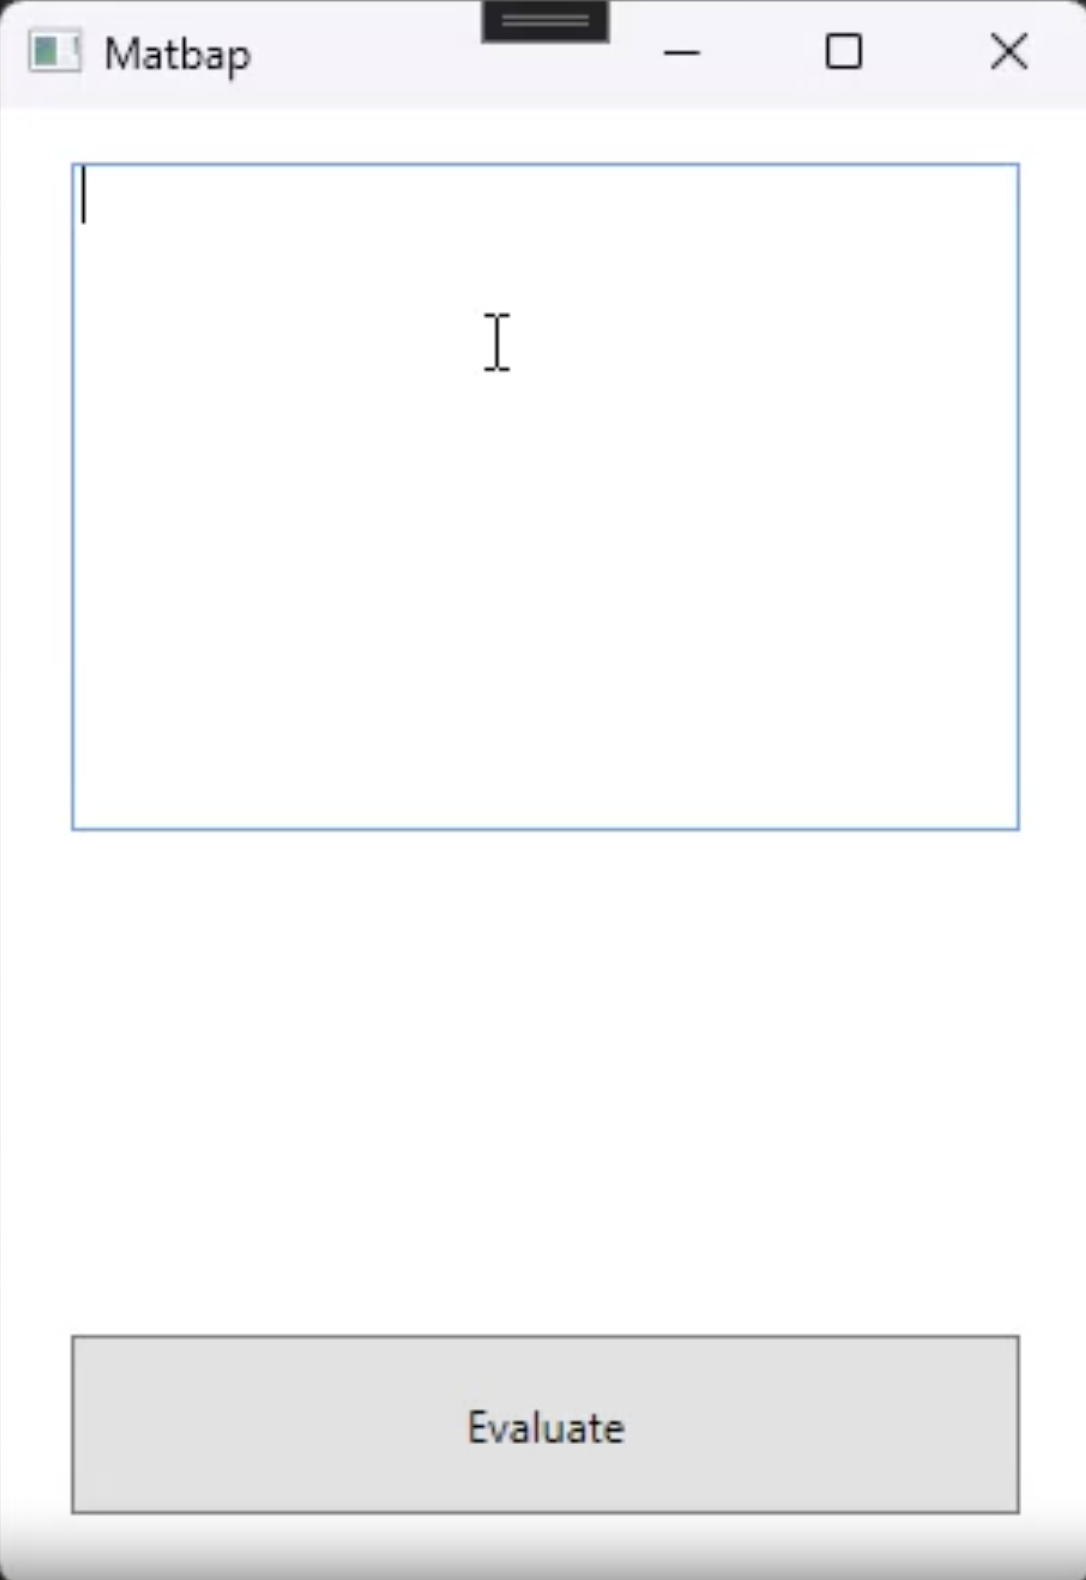
\includegraphics[scale=0.3 ]{Basic GUI.png}
\caption{Our first basic GUI}
\label{basicgui}
\end{center}
\end{figure}

\section{Updated GUI with Help Window}
\label{helpgui}

\section{Visualise parse tree GUI}
\begin{figure}[H]
\begin{center}
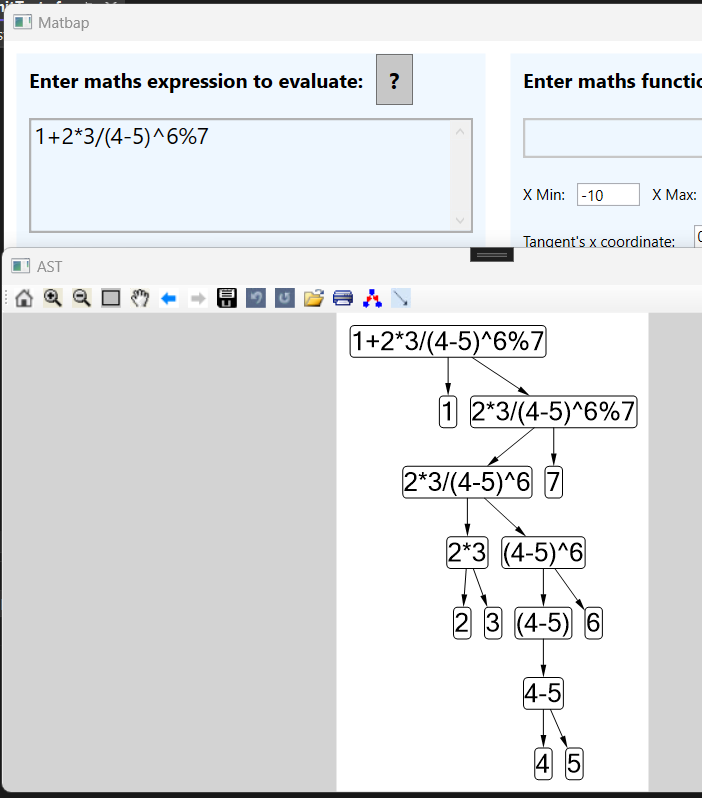
\includegraphics[scale=0.3 ]{VisualuseASTGUI.png}
\caption{AST visualistion}
\label{basicgui}
\end{center}
\end{figure}

\section{GUI with multiple plots, clear and plotted functions table}
\begin{figure}[H]
\begin{center}
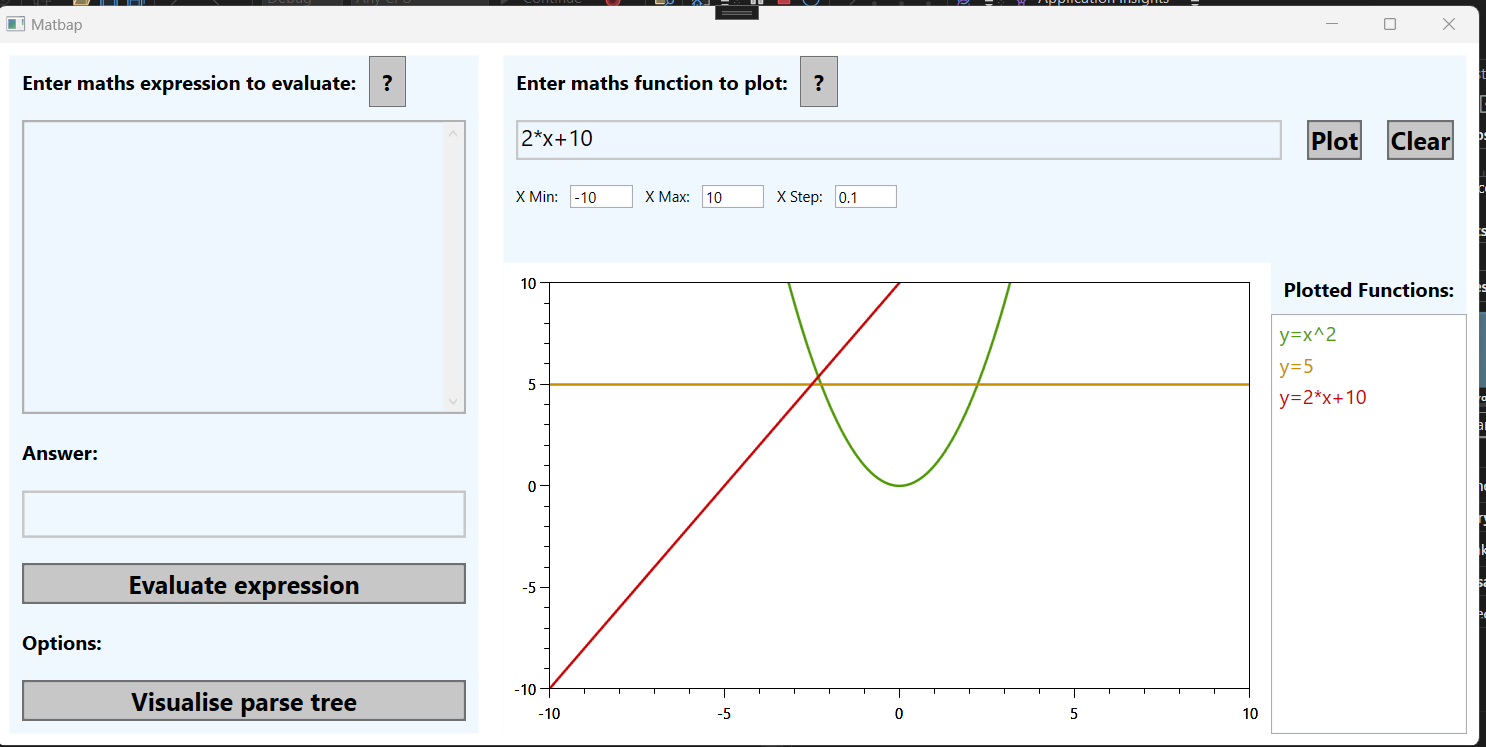
\includegraphics[scale=0.3 ]{MultiplePlotsGUI.png}
\caption{Reworked GUI}
\label{basicgui}
\end{center}
\end{figure}


\chapter{Algorithms}
\label{app:algorithms}

\begin{algorithm}
\begin{algorithmic}[1]
\caption{Recursively differentiate an AST}
\label{algorithm-differentiate}
\STATE An AST node.
\STATE A variable with respect to differentiate to.
\STATE A Lookup Table(LUT) for trigonometric and logarithmic functions.
    \IF {$node$ is a constant}
        \STATE \Return 0
    \ELSIF {$node$ is a variable}
        \STATE \Return 1
    \ELSIF {$node$ is a not variable we differentiate with respect to}
        \STATE \Return 0
    \ELSIF {$node$ is a binary operation}
        \IF {$node$ is addition or subtraction}
            \STATE $u \gets$ {Differentiate}({$node.left$})
            \STATE $v \gets$ {Differentiate}({$node.right$})
            \STATE \RETURN u $\pm$ v
        \ELSIF {$node$ is multiplication}
            \STATE $u \gets$ {Differentiate}({$node.left$})
            \STATE $v \gets$ {Differentiate}({$node.right$})
            \STATE \RETURN u $\times$ $node.right$ + v $\times$ $node.left$ 
        \ELSIF {$node$ is division}
            \STATE $u \gets$ {Differentiate}({$node.left$})
            \STATE $v \gets$ {Differentiate}({$node.right$})
            \STATE \RETURN $(u \times node.right - v \times node.left) / (node.right)^2$
        \ELSIF {$node$ is a power}
            \STATE $u \gets$ {Differentiate}({$node.left$})
            \STATE $v \gets$ {Differentiate}({$node.right$})
            \STATE \RETURN $node.right$ $\times$ $node.base^{node.right-1}$ $\times$ {Differentiate}({$node.base$})
        \ENDIF
    \ELSIF {$node$ is a trigonometric or logarithmic function}
        \STATE $u \gets node.innerNode$
        \STATE $du \gets$ {Differentiate}({$u$})
        \STATE $outerDerivative \gets$ {LUT}({$node.function$})
        \STATE \RETURN $outerDerivative(u) \times du$
    \ENDIF
    
\end{algorithmic}
\end{algorithm}

\chapter{Links}
\label{app:links}
\section{Jira Board}
https://liamfarese.atlassian.net/jira/software/projects/AP/boards/2
\label{ap-jira-link}

\section{GitHub repository}
https://github.com/IgorSteps/matbap
\label{github-repo}

\end{document}

